\chapter{HASIL DAN PEMBAHASAN}
\section{Hasil Perancangan Sistem}
Sistem deteksi kecacatan kontainer yang dikembangkan pada penelitian
ini dirancang untuk bekerja secara otomatis dengan menggunakan kamera
sebagai sensor utama dan lengan robot sebagai aktuator. Proses
diawali oleh model YOLO yang mendeteksi keberadaan kontainer dari
citra hasil tangkapan kamera. Jika objek kontainer berhasil
terdeteksi, citra tersebut dianalisis oleh model \textit{autoencoder}
untuk mengklasifikasikan apakah kontainer mengalami kecacatan.
Berdasarkan hasil klasifikasi, mikrokontroler mengendalikan motor
\textit{servo} untuk menggerakkan lengan robot guna menyortir
kontainer ke dalam kategori cacat atau tidak cacat. Secara paralel,
sensor PIR digunakan untuk menghitung jumlah total kontainer pada
masing-masing kategori. Data ini kemudian dikirim (melalui metode
POST) ke \textit{web server} untuk divisualisasikan pada sisi klien
melalui tampilan \textit{website}. Desain sistem yang telah dirancang
diilustrasikan pada Gambar \ref{fig:rancang-sistem}.

\begin{figure}[H]
  \centering
  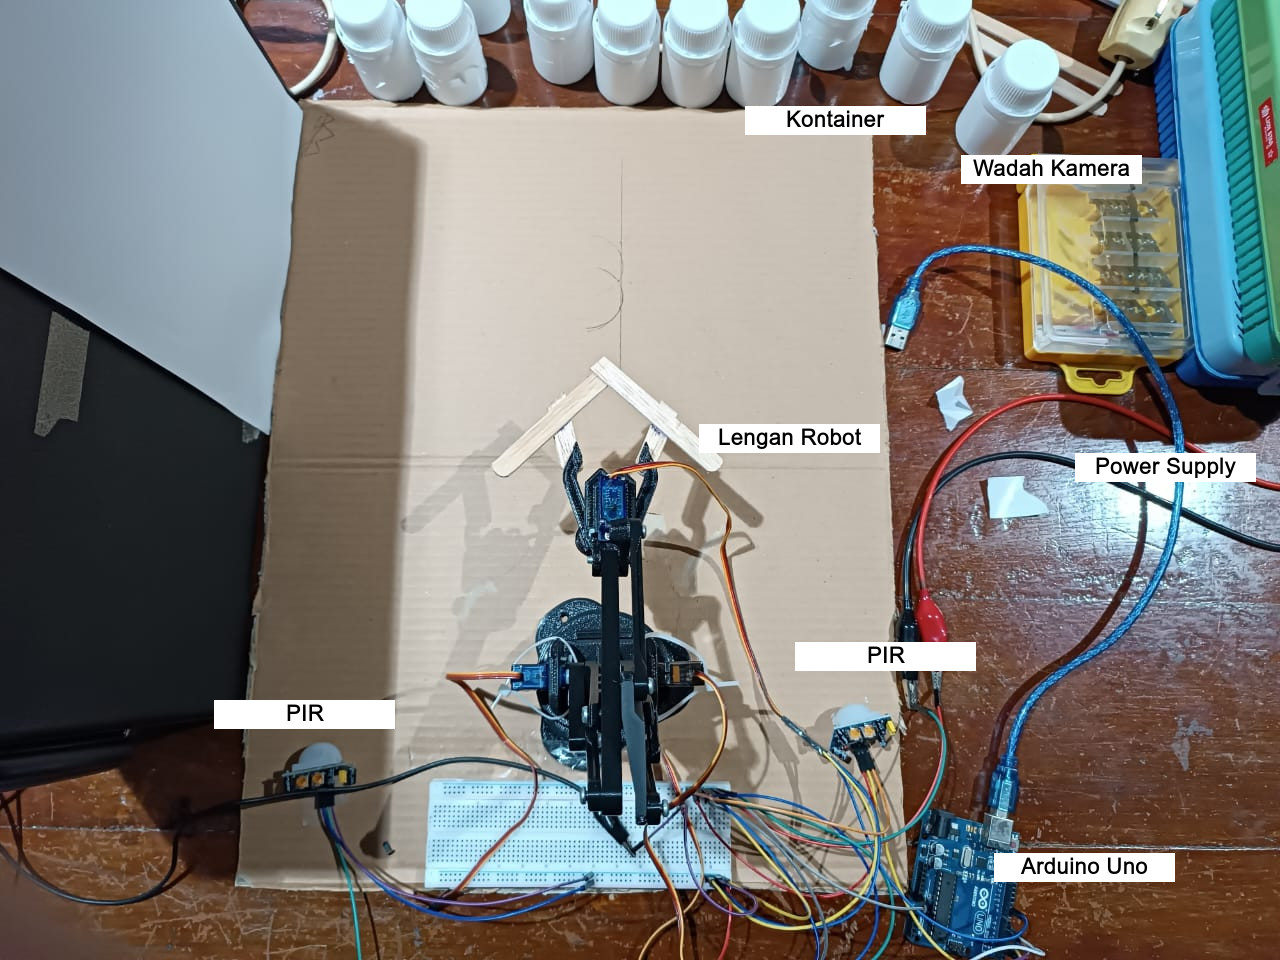
\includegraphics[width=\textwidth]{gambar/rancang_sistem.jpg}
  \caption{Hasil perancangan sistem}
  \label{fig:rancang-sistem}
\end{figure}
\vspace{-1em}

\vspace{1em}

\section{Hasil Perancangan Model YOLO}
\subsection{\textit{Dataset} dan \textit{Preprocessing}}
Tahap awal penelitian adalah pengumpulan data primer berupa citra
kontainer kimia menggunakan kamera. Proses akuisisi ini dilakukan
untuk membangun  sebuah \textit{dataset} kustom yang mampu merepresentasikan
objek target secara akurat. Total citra mentah yang berhasil
dikumpulkan berjumlah 463 citra yang diambil dari berbagai posisi dan
sudut pandang untuk memastikan model dapat mengenali objek dalam
berbagai kondisi. \textit{Dataset} kemudian dibagi menjadi 395 citra
untuk data latih dan 68 citra data validasi. Distribusi pembagian dataset
disajikan pada Tabel \ref{tab:pembagian-dataset}.

\begin{table}[H]
  \caption{Distribusi pembagian \textit{dataset}}
  \label{tab:pembagian-dataset}
  \vspace{-1em}
  \centering
  \begin{tabular}{ccc}
    \toprule
    \textbf{Kategori} & \textbf{Jumlah Gambar} & \textbf{Persentase} \\
    \midrule
    Data Latih & 395 & 85,3\% \\
    Data Validasi & 68 & 14,7\% \\
    Total Data & 463 & 100\% \\
    \bottomrule
  \end{tabular}
\end{table}

Setelah akuisisi data, dilakukan anotasi citra untuk
memberikan \textit{bounding box} dan label kelas pada setiap objek yang
terdeteksi di dalam citra. Proses ini penting karena arsitektur YOLO
dirancang untuk secara simultan memprediksi letak objek dan kelasnya,
sehingga memerlukan data berlabel \citep{19,20}. Sebanyak 463 citra
kontainer telah dianotasi secara manual. Contoh hasil anotasi dapat
dilihat pada Gambar \ref{fig:yolo-anotasi}.

\begin{figure}[H]
  \centering
  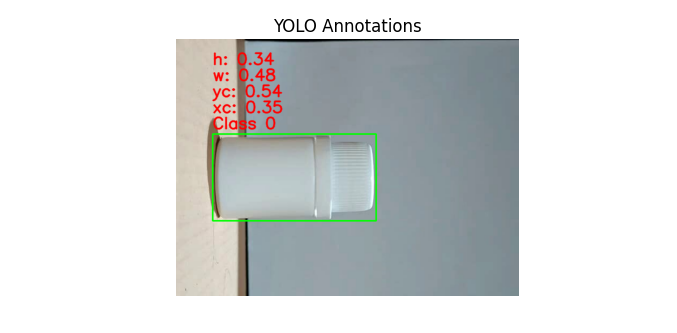
\includegraphics[width=0.7\textwidth]{gambar/anotasi.png}
  \caption{Salah satu data \textit{train} dengan labelnya}
  \label{fig:yolo-anotasi}
\end{figure}
\vspace{-1em}

\vspace{1em}

\subsection{Hasil Pelatihan Model}
Dalam penelitian ini, metrik utama yang digunakan untuk mengevaluasi
performa model YOLO adalah mAP. Metrik ini penting untuk menilai
seberapa akurat model dalam mendeteksi objek
seingga lengan robot dapat melakukan penyortiran secara tepat. Nilai
mAP dihitung berdasarkan rata-rata \textit{Average Precision} (AP), yang
merupakan gabungan antara \textit{precision} dan \textit{recall}
untuk setiap kelas \citep{21}.

Untuk menentukan apakah sebuah prediksi tergolong benar (\textit{True
Positive}) atau salah (\textit{False Positive}), digunakan metrik
\textit{Intersection over Union} (IoU). IoU yaitu rasio antara
\textit{bounding box} prediksi ($BB_{predict}$) dengan
\textit{bounding box} sebenarnya ($BB_{ground}$), dengan nilai
mendekati 1 menunjukkan prediksi yang sangat akurat \citep{22}.
Semakin mendekati 1, berarti prediksi semakin akurat dan sesuai
dengan objek sebenarnya. IoU dihitung menggunakan persamaan:
\begin{equation}
  IoU = \frac{|BB_{predict} \cap
  BB_{ground}|}{|BB_{predict} \cup BB_{ground}|}
\end{equation}
\indent
Selanjutnya, \textit{precision} mengukur proporsi prediksi positif
yang benar (\textit{True Positive}) terhadap seluruh prediksi positif
(TP + \textit{False Positive}), sedangkan \textit{recall} atau
\textit{true positive rate} mengukur seberapa banyak objek yang
benar-bernar terdeteksi \citep{23}. \textit{Precision} dan
\textit{recall} dapat dihitung menggunakan persamaan:
\begin{equation}
  Precision = \frac{TP}{TP + FP}, \quad
  Recall = \frac{TP}{TP + FN}
\end{equation}
\indent
Karena model YOLO dalam penelitian ini hanya memprediksi satu kelas
yaitu kontainer kimia, maka nilai mAP setara dengan nilai AP. Nilai
AP dihitung sebagai rata-rata \textit{precision} di seluruh rentang nilai
\textit{recall} (0 hingga 1) \citep{24}, sebagaimana dirumuskan dalam
Persamaan 3, di mana P adalah \textit{precision} dan r adalah \textit{recall}.
\begin{equation}
  AP = \int_{0}^{1} P(r) \,dr
\end{equation}
\indent
Proses pelatihan model YOLO dilakukan di platform \textit{Google
Colaboratory} selama 50 \textit{epoch} menggunakan \textit{batch
size} 16 dan \textit{optimizer} Adam. Ringkasan hasil pelatihan
setiap 10 \textit{epoch} disajikan pada Tabel \ref{tab:yolo-train}.
\begin{table}[H]
  \caption{Proses \textit{training} model YOLO}
  \label{tab:yolo-train}
  \vspace{-1em}
  \centering
  \small
  \begin{tabular}{c p{1.5cm} p{1.5cm} p{1.5cm} p{1.5cm} p{1.5cm} p{1.5cm}}
    \toprule
    \textbf{Epoch} & \textbf{Train/Box Loss} & \textbf{Train/Class Loss}
    & \textbf{Train/DFL Loss} & \textbf{Val/Box Loss}
    & \textbf{Val/Class Loss} & \textbf{Val/DFL Loss} \\
    \midrule
    0  & 0,5946 & 1,9374 & 0,9706 & 0,4709 & 2,5029 & 0,8990 \\
    10 & 0,4333 & 0,4356 & 0,8713 & 0,3052 & 0,3758 & 0,8262 \\
    20 & 0,3286 & 0,2935 & 0,8510 & 0,3342 & 0,2105 & 0,8448 \\
    30 & 0,2821 & 0,2328 & 0,8390 & 0,2418 & 0,1566 & 0,8244 \\
    40 & 0,2267 & 0,1776 & 0,8010 & 0,2209 & 0,1386 & 0,8201 \\
    50 & 0,2016 & 0,1546 & 0,7993 & 0,2003 & 0,1163 & 0,8156 \\
    \bottomrule
  \end{tabular}
  \normalsize
\end{table}
Nilai \textit{loss} pada data latih dan validasi secara umum
menunjukkan tren menurun, mengindikasikan bahwa model berhasil
menyesuaikan parameter internalnya dengan data. Pada
\textit{Train/Box Loss}, terjadi penurunan
signifikan dari 0,5946 pada \textit{epoch} ke-0 menjadi 0,2016 pada
\textit{epoch} ke-50, yang menunjukkan peningkatan akurasi deteksi
posisi objek. Penurunan signifikan juga terlihat pada \textit{Train/Class
Loss} dan \textit{Train/DFL Loss}, serta pada seluruh komponen
\textit{loss} di data validasi. Penurunan konsisten ini menunjukkan
bahwa model memiliki kemampuan generalisasi yang
baik pada data validasi.

Meskipun demikian, nilai \textit{loss} saja tidak cukup untuk menilai
keseluruhan performa model. Oleh karena itu, digunakan pula metrik
mAP, seperti mAP@50 dan mAP@50-95, untuk
mengevaluasi ketepatan deteksi: mAP@50 berarti evaluasi dilakukan
dengan ambang IoU 50\% yang cenderung lebih longgar, sedangkan
mAP@50-95 adalah rata-rata mAP pada ambang IoU dari 50\% hingga 95\%
dengan interval 5\%, sehingga lebih ketat. Hasil pengukuran mAP pada
tiap \textit{epoch} dapat dilihat pada Gambar \ref{fig:map}.

\begin{figure}[H]
  \centering
  % First image
  \begin{minipage}[]{\textwidth}
    \centering
    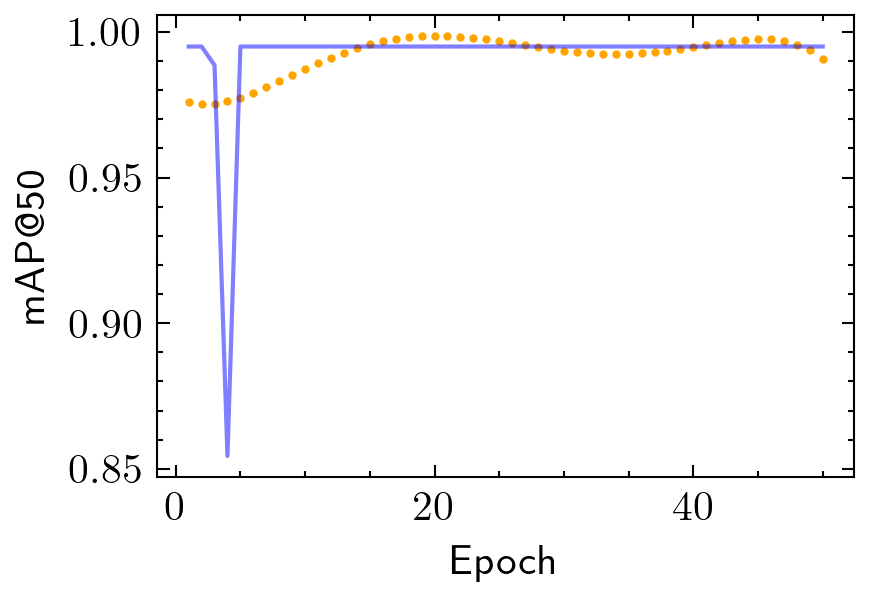
\includegraphics[width=0.625\textwidth]{gambar/map50.png}
    (a)
  \end{minipage}
  \vspace{1em}

  % Second image
  \begin{minipage}{\textwidth}
    \centering
    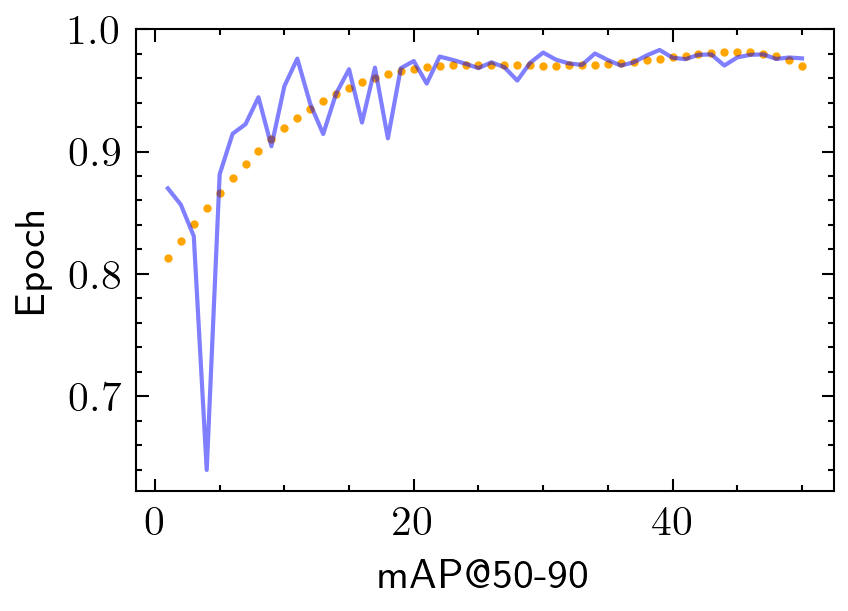
\includegraphics[width=0.625\textwidth]{gambar/map5090.png}
    (b)
  \end{minipage}
  \caption{Grafik tren mAP: (a) mAP@50, (b) mAP@50-95}
  \label{fig:map}
  \vspace{-1em}
\end{figure}

Grafik (a) menunjukkan bahwa model dengan cepat mencapai nilai mAP
tinggi pada ambang 50\%, bahkan dalam 10-15 \textit{epoch} pertama.
Grafik (b) menunjukkan tren yang lebih lambat dan bertahap,
mengindikasikan proses penyempurnaan presisi dan akurasi posisi
\textit{bounding box}. Secara keseluruhan, nilai mAP yang tinggi pada
kedua metrik diakhir
pelatihan menunjukkan bahwa model yang dihasilkan tidak hanya mampu
mendeteksi objek, tetapi juga mampu menentukan batas objek secara akurat.
Contoh hasil prediksi model YOLO terhadap data validasi disajikan
pada Gambar \ref{fig:yolo-validasi}.

\begin{figure}[H]
  \centering
  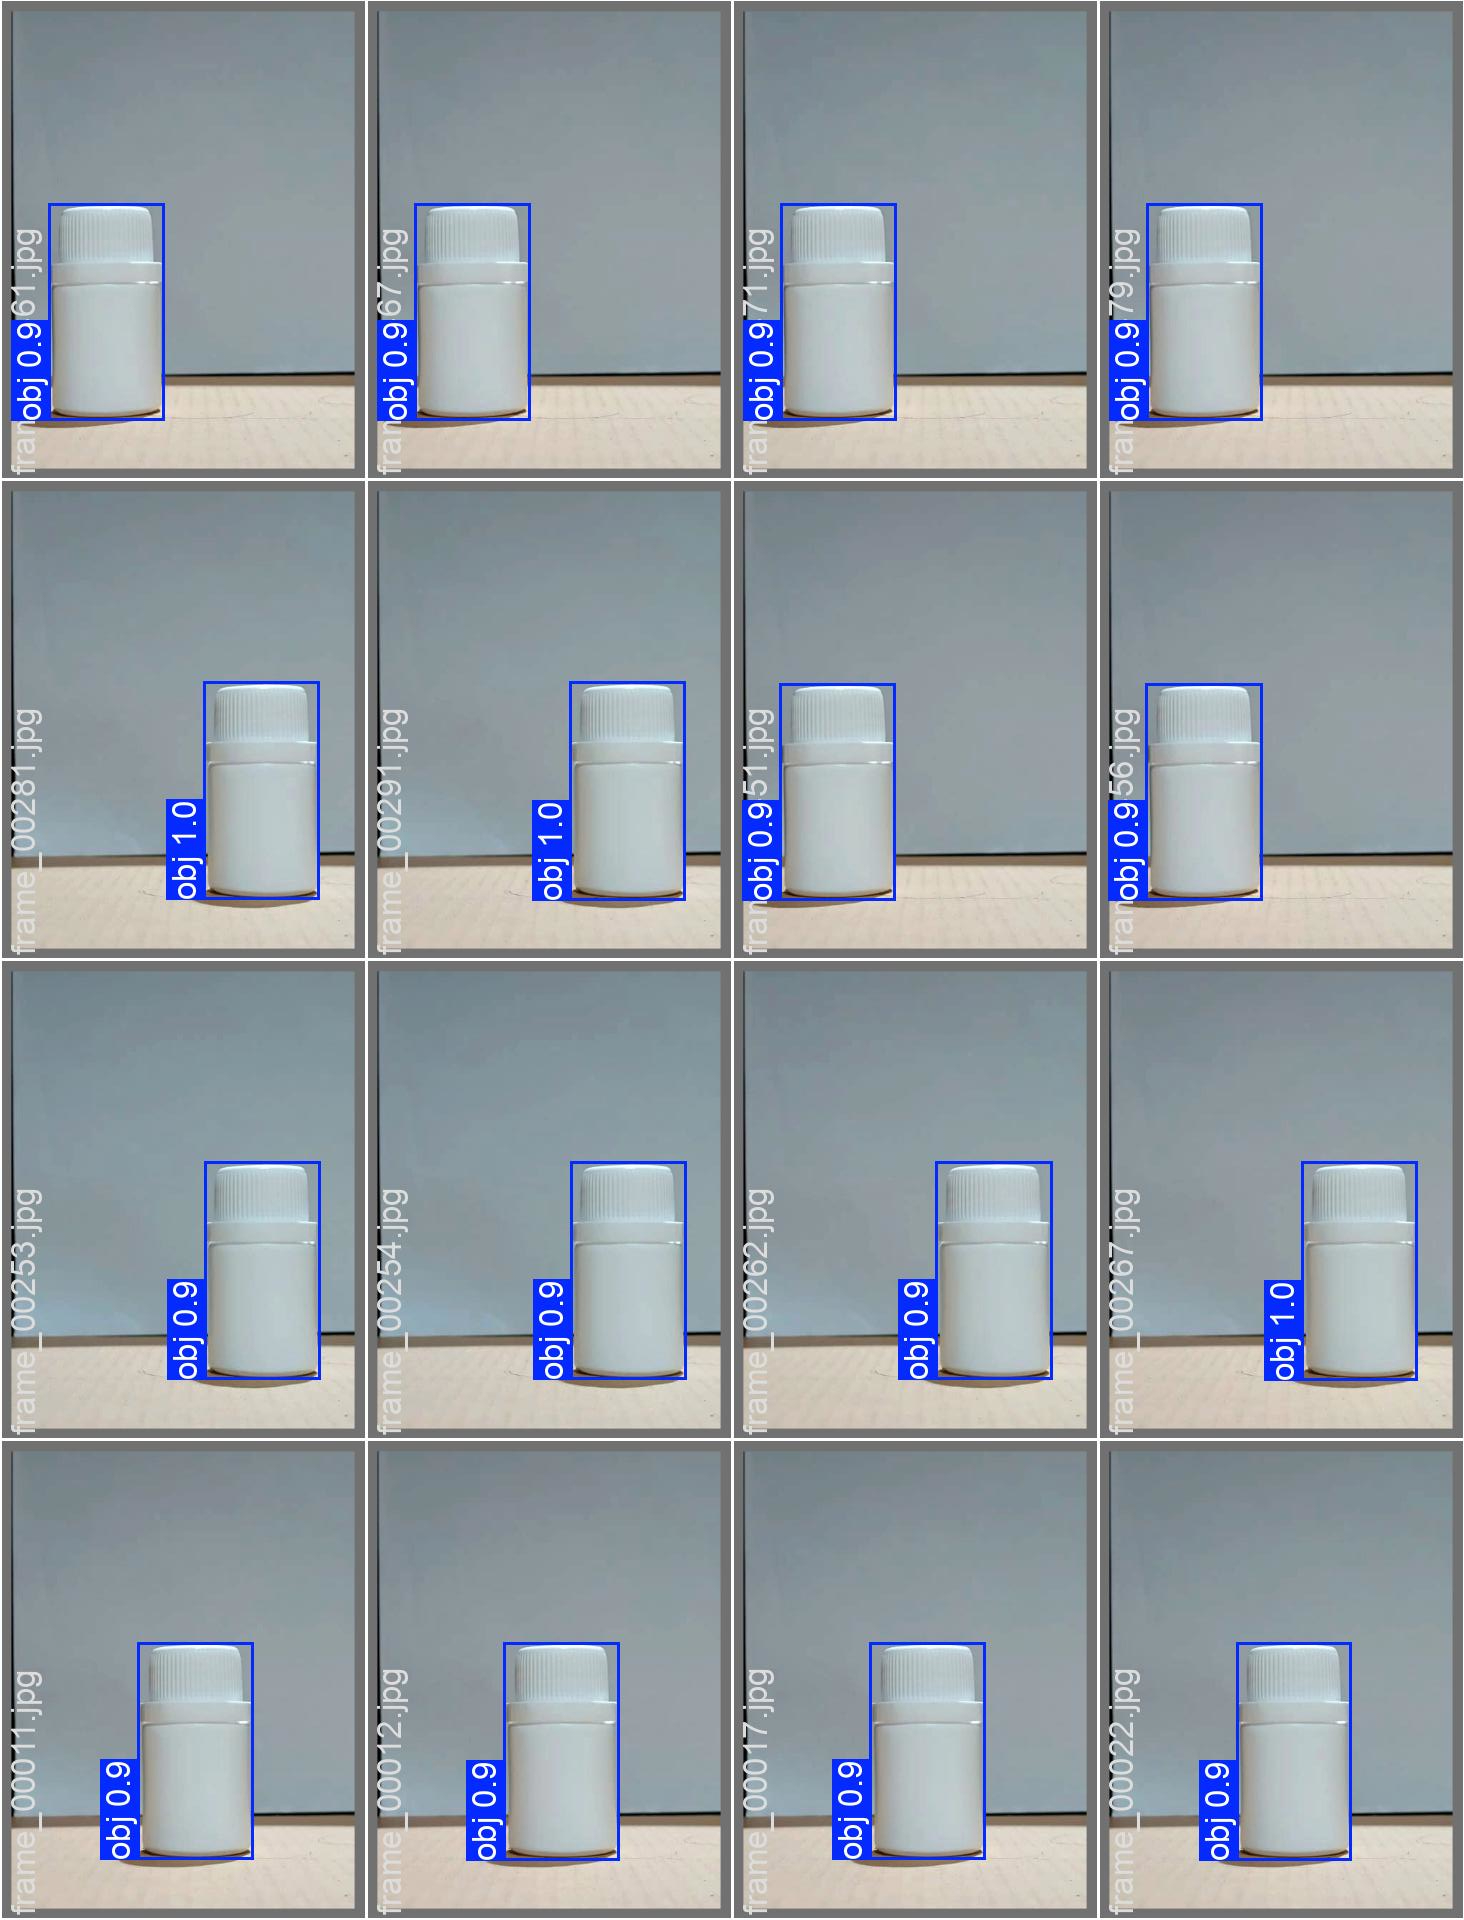
\includegraphics[width=0.93\textwidth]{gambar/yolo_validasi.jpg}
  \caption{Hasil prediksi YOLO pada data validasi}
  \label{fig:yolo-validasi}
\end{figure}
\vspace{-1em}

\vspace{1em}

\section{Hasil Perancangan Model Deteksi Kecacatan}
\subsection{Arsitektur Variational Autoencoder}
\textit{Variational autoencoder} (VAE) merupakan pengembangan dari
\textit{autoencoder}, yaitu arsitektur \textit{neural network}
yang berfungsi untuk mengekstraksi fitur laten dari data. Perbedaan
utama VAE dibandingkan \textit{autoencoder} konvensional adalah
pendekatannya yang berbasis Bayesian, di mana vektor laten ($z$)
dipaksa mengikuti distribusi probabilitas terstruktur, biasanya
distribusi Gaussian. Secara operasional, bagian \textit{encoder} VAE
($q_{\phi}(z \mid x)$) tidak hanya mengompresi data masukan ($x$),
tetapi juga memetakannya ke dalam parameter statistik: yaitu vektor
rata-rata (\textit{mean}) dan vektor varians (\textit{log-varians}).
Kemudian, sebuah vektor laten ($z$) diambil dari distribusi dan
diteruskan ke \textit{decoder} ($p_{\theta}(x \mid z)$) untuk
merekonstruksi kembali data masukan \citep{25}. Arsitektur
\textit{variational autoencoder} yang
digunakan pada penelitian ini dapat dilihat pada Gambar
\ref{fig:arsitektur-autoencoder}.

\begin{figure}[H]
  \centering
  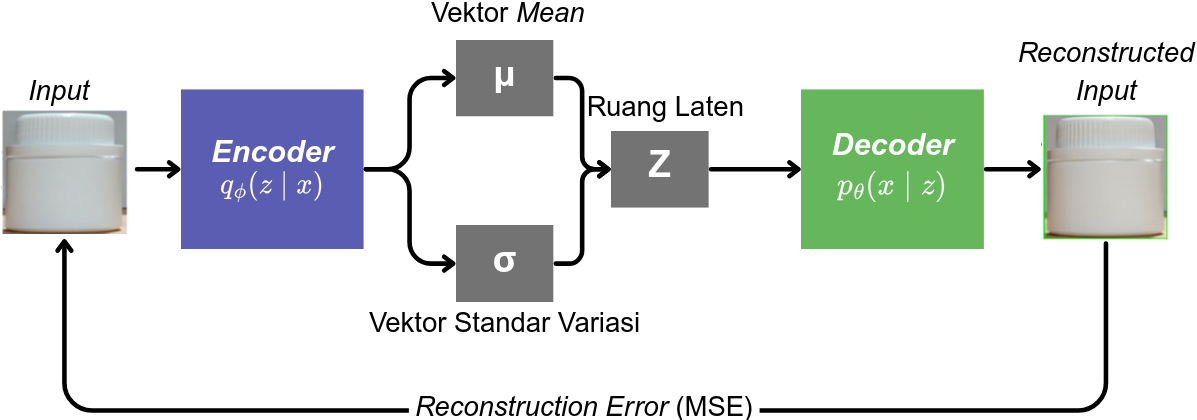
\includegraphics[width=\textwidth]{gambar/arsitektur_autoencoder.png}
  \caption{Arsitektur \textit{variational autoencoder}}
  \label{fig:arsitektur-autoencoder}
\end{figure}
\vspace{-1em}

Arsitektur VAE dirancang untuk memproses citra berukuran 128 $\times$
128 dengan tiga kanal warna (RGB). Bagian \textit{encoder}
terdiri atas lima lapisan
\textit{convolutional} berurutan, masing-masing diikuti fungsi
aktivasi ReLU yang bertugas menurunkan
resolusi fitur spasial dan mengekstraksi fitur penting hingga
menghasilkan representasi akhir berdimensi (512, 4, 4). Representasi
ini kemudian diproyeksikan menjadi dua vektor statistik, yaitu vektor
\textit{mean} dan vektor \textit{log-varians}, yang bersama-sama
membentuk distribusi
Gaussian multivariat sebagai ruang laten. Setelah proses pengambilan
sampel dari ruang laten, vektor z diteruskan ke \textit{decoder} yang
memproyeksikan kembali representasi tersebut melalui lapisan linear
dan beberapa lapisan \textit{transpose convolutional} (dekonvolusi) untuk
mengembalikan ukuran citra ke dimensi semula. Fungsi aktivasi
sigmoid pada lapisan \textit{output} memastikan nilai piksel berada pada
rentang [0, 1], sehingga citra hasil rekonstruksi dapat
diinterpretasikan sebagai citra valid.

\vspace{1em}

\subsection{\textit{Dataset} dan \textit{Preprocessing}}
Tahap ini diawali dengan pengumpulan data primer berupa citra
kontainer kimia menggunakan kamera. Tujuannya adalah membangun
\textit{dataset} kustom yang dapat merepresentasikan objek target secara
spesifik. Total citra mentah yang berhasil dikumpulkan berjumlah 3005
citra, yang seluruhnya digunakan sebagai data latih. Sebelum
digunakan untuk pelatihan \textit{autoencoder}, seluruh citra diproses
terlebih dahulu menggunakan model YOLO untuk mendeteksi serta
memotong (\textit{cropping}) area kontainer secara
otomatis. Hal ini bertujuan agar hanya bagian penting dari kontainer
yang diproses lebih lanjut, sehingga model \textit{autoencoder} dapat
secara optimal mempelajari karakteristik visual kontainer. Contoh
salah satu citra data latih ditunjukkan pada Gambar \ref{fig:ae-data}.

\begin{figure}[H]
  \centering
  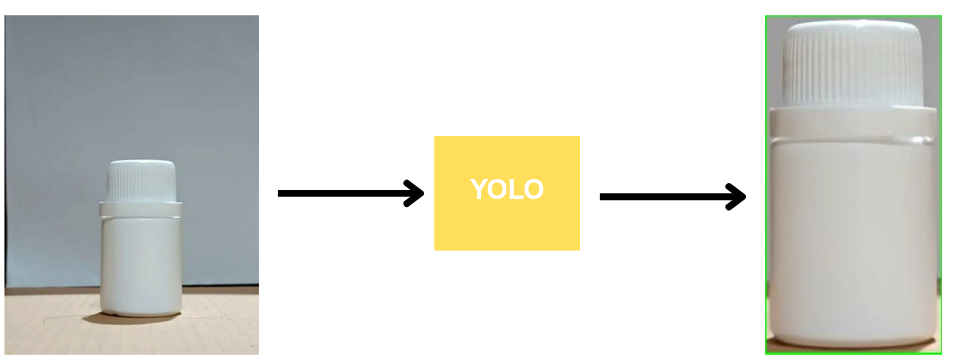
\includegraphics[width=\textwidth]{gambar/ae_data.png}
  \caption{Salah satu data latih model \textit{autoencoder}}
  \label{fig:ae-data}
\end{figure}
\vspace{-1em}

Karena \textit{autoencoder} termasuk dalam kategori
\textit{unsupervised learning},
maka data tidak memerlukan label atau anotasi manual. \textit{Dataset} ini
hanya terdiri dari citra kontainer dalam kondisi baik (tanpa
kerusakan/cacat visual), sehingga model \textit{autoencoder} dapat mempelajari
distribusi visual normal secara optimal. Dengan demikian, saat
digunakan pada data yang mengandung cacat model akan menunjukkan
perbedaan yang mencolok antara citra asli dan hasil rekonstruksi yang
menjadi dasar untuk mendeteksi anomali.

\vspace{1em}

\subsection{Hasil Pelatihan Model}
Fungsi \textit{loss} pada VAE didasarkan pada prinsip
\textit{Evidence Lower Bound}
(ELBO) yang bertujuan mengoptimalkan model probabilistik dengan
mengatasi kendala distribusi posterior yang tidak dapat dihitung
secara langsung. Fungsi \textit{loss} VAE terdiri dari dua komponen utama: (1)
\textit{reconstruction loss}, yang mengukur selisih antara citra asli (x) dan
citra hasil rekonstruksi dari vektor laten z, dan (2) \textit{regularization
term} berupa divergensi Kullback-Leibler (KL) yang mengukur sejauh
mana distribusi posterior hasil \textit{encoder} menyimpang dari distribusi
Gaussian standar \citep{26}. Fungsi \textit{loss} VAE dirumuskan
sebagai berikut:
\begin{equation}
  \mathcal{L}(\theta, \phi; x) = \mathbb{E}{q\phi(z|x)}[\log
  p_\theta(x|z)] - D_{KL}(q_\phi(z|x) \parallel p_\theta(z))
\end{equation}
\indent
Model CVAE dilatih
menggunakan komputer dengan GPU NVIDIA GeForce RTX 3050 8GB VRAM
untuk memanfaatkan kemampuan komputasi paralel CUDA. Proses pelatihan
dilakukan selama 100 \textit{epoch} dengan
\textit{batch size} 64
dan \textit{optimizer} Adam. Nilai \textit{loss} setiap 10
\textit{epoch} ditampilkan pada Tabel \ref{tab:training-autoencoder}.

\begin{table}[H]
  \caption{Proses \textit{training} model model \textit{convolutional
  variational autoencoder}}
  \label{tab:training-autoencoder}
  \vspace{-1em}
  \centering
  \begin{tabular}{cc}
    \toprule
    \textbf{Epoch} & \textbf{Loss} \\
    \midrule
    1 & 837,7615 \\
    10 & 30,5440 \\
    20 & 22,6941 \\
    30 & 18,5220 \\
    40 & 15,0172 \\
    50 & 11,9098 \\
    60 & 9,8593 \\
    70 & 8,7772 \\
    80 & 7,3923 \\
    90 & 7,1070 \\
    100 & 6,8338 \\
    \bottomrule
  \end{tabular}
\end{table}
Penurunan nilai \textit{loss} selama proses pelatihan menunjukkan bahwa model
CVAE secara bertahap berhasil mempelajari pola visual dari kontainer
normal. Dengan semakin kecilnya nilai \textit{loss}, model menunjukkan
kemampuan yang semakin baik dalam merekonstruksi citra tanpa cacat,
sehingga mampu membedakan citra cacat secara signifikan. Hasil
rekonstruksi ditampilkan pada Gambar \ref{fig:autoencoder-test}.

\begin{figure}[H]
  \centering
  % First image
  \begin{minipage}{\textwidth}
    \centering
    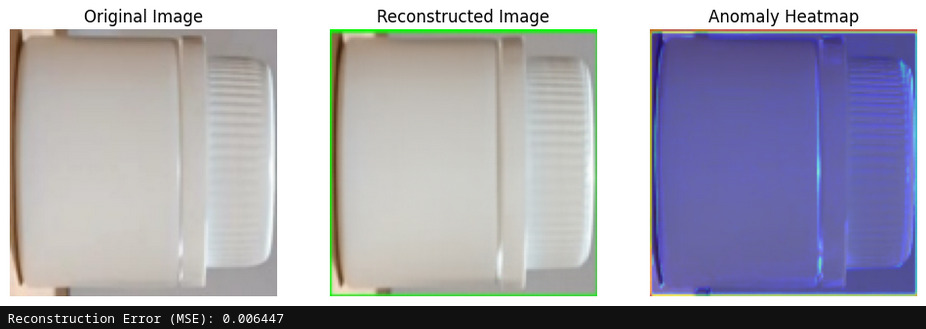
\includegraphics[width=\textwidth]{gambar/kontainer_bagus.jpeg}
    (a)
  \end{minipage}
  \vspace{1em}

  % Second image
  \begin{minipage}{\textwidth}
    \centering
    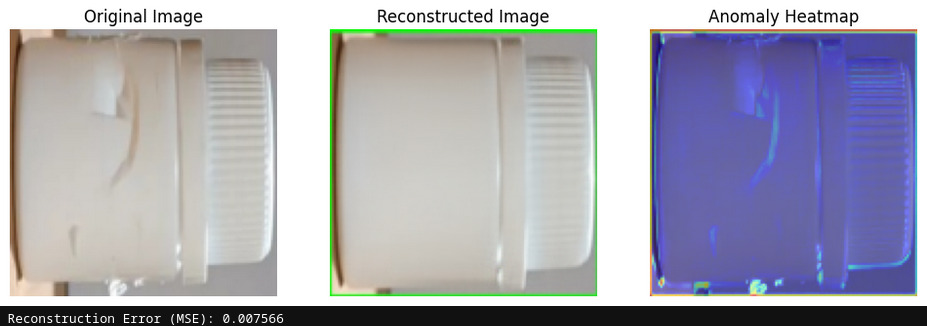
\includegraphics[width=\textwidth]{gambar/kontainer_cacat.jpeg}
    (b)
  \end{minipage}
  \caption{Hasil prediksi kecacatan: (a) Kontainer normal, (b)
  kontainer cacat}
  \label{fig:autoencoder-test}
  \vspace{-1em}
\end{figure}

Dari gambar di atas, diketahui bahwa nilai rekonstruksi
\textit{error} untuk kontainer
normal adalah 0,006447, sedangkan untuk kontainer cacat sebesar
0,007566. Selisih ini menunjukkan bahwa model mampu membedakan citra
cacat dari normal normal berdasarkan tingkat kesalahan rekonstruksi.

\vspace{1em}

\subsection{Penentuan Ambang Batas Kecacatan}
Penentuan ambang batas merupakan langkah penting dalam memastikan
sistem deteksi cacat dapat secara akurat membedakan kontainer cacat
dan tidak cacat. Tanpa ambang batas yang tepat, sistem beresiko
menghasilkan banyak kesalahan klasifikasi yang tinggi. Dalam
penelitian ini, digunakan metrik \textit{Mean Squared Error} (MSE) untuk
mengukur perbedaan antara citra asli dan hasil rekonstruksi.

MSE menghitung rata-rata selisih kuadrat antara piksel citra asli
(\textit{input}) dengan piksel citra hasil rekonstruksi
(\textit{output}). Semakin
kecil nilai MSE, semakin mirip citra hasil rekonstruksi dengan citra
aslinya, yang berarti model berhasil meminimalkan distorsi
\citep{27}. MSE dirumuskan sebagai berikut:

\begin{equation}
  MSE = \frac{1}{n} \sum_{i=1}^{n} (x_i - \hat{x}_i)^2
\end{equation}

Pengujian dilakukan terhadap 20 citra, terdiri dari 10 kontainer
normal dan 10 gambar kontainer cacat. Dari pengujian ini diperoleh
distribusi nilai MSE masing-masing citra untuk dianalisis lebih
lanjut. Hasil perhitungan MSE pada 20 gambar uji tersebut dirangkum
pada Tabel \ref{tab:error-samples}.

\begin{table}[H]
  \centering
  \caption{Nilai \textit{error} untuk setiap sampel}
  \label{tab:error-samples}
  \begin{tabular}{ccc}
    \toprule
    \textbf{No} & \textbf{Error} & \textbf{Kategori} \\
    \midrule
    1  & 0,006737 & Normal \\
    2  & 0,006828 & Normal \\
    3  & 0,007091 & Normal \\
    4  & 0,006997 & Normal \\
    5  & 0,006610 & Normal \\
    6  & 0,006795 & Normal \\
    7  & 0,006872 & Normal \\
    8  & 0,006725 & Normal \\
    9  & 0,006873 & Normal \\
    10 & 0,006817 & Normal \\
    11 & 0,007432 & Cacat \\
    12 & 0,007455 & Cacat \\
    13 & 0,008369 & Cacat \\
    14 & 0,007183 & Cacat \\
    15 & 0,007653 & Cacat \\
    16 & 0,008856 & Cacat \\
    17 & 0,007531 & Cacat \\
    18 & 0,007624 & Cacat \\
    19 & 0,007457 & Cacat \\
    20 & 0,008424 & Cacat \\
    \bottomrule
  \end{tabular}
\end{table}

Dari tabel di atas, nilai MSE untuk kontainer normal berkisar 0,0067
sedangkan nilai untuk kontainer cacat secara konsisten lebih tinggi.
Hal ini menunjukkan bahwa perbedaan rekonstruksi pada citra cacat
lebih besar, menandakan kegagalan model untuk merekonstruksi fitur
yang tidak dikenalnya. Untuk mnentukan ambang batas optimal,
digunakan metode \textit{Receiver Operating Characteristic} (ROC)
yang memplot \textit{true positive rate} (recall) terhadap
\textit{false positive rate} (1 – \textit{specificity}) \citep{28}.
Nilai ambang terbaik ditentukan dengan memaksimalkan statistik Youden
J yang dirumuskan sebagai:

\begin{equation}
  J = \textit{True Positive Rate} - \textit{False Positive Rate}
\end{equation}

Kurva ROC dari hasil pengujian ditampilkan pada Gambar \ref{fig:roc}
digunakan sebagai metode analisis untuk mengevaluasi performa model
deteksi cacat pada kontainer kimia dalam penelitian ini. Kurva ROC dibuat
dengan memplot nilai 1 - \textit{specificity} (\textit{false positive
rate}) pada sumbu-x dan \textit{recall} (\textit{true positive rate})
pada sumbu-y untuk setiap nilai ambang batas yang diuji.
\textit{Specificity} sendiri adalah ukuran seberapa baik model dalam
mengenali data negatif secara benar. Nilai ambang batas terbaiki
ditentukan dengan memaksimalkan statistik Youden J, yang dirumuskan
pada Persamaan 6.

\begin{figure}[H]
  \centering
  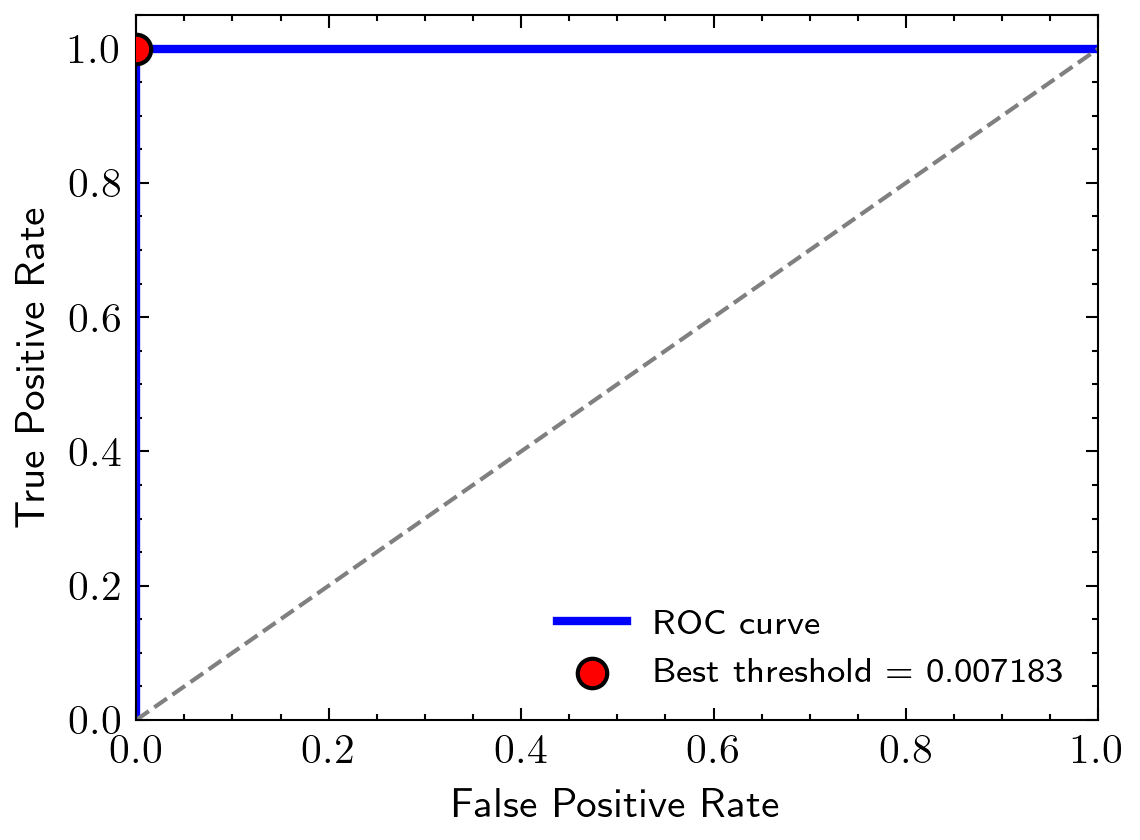
\includegraphics[width=\textwidth]{gambar/roc.png}
  \caption{Kurva ROC}
  \label{fig:roc}
\end{figure}
\vspace{-1em}

Kurva ROC menunjukkan bahwa model memiliki performa yang sangat baik,
dengan garis mendeteksi sudut kiri atas. Berdasarkan kurva, diperoleh
nilai ambang optimal ditunjukkan oleh garis biru yang mendekati titik
sudut kiri atas. Berdasarkan perhitungan, ambang batas optimal
sebesar 0,007183, ditandai dengan lingkaran merah pada grafik. Nilai
ini digunakan sebagai batas akhir dalam klasifikasi kontainer cacat
dan tidak cacat, guna memaksimalkan sensitivitas sekaligus
meminimalkan kesalahan deteksi positif.

\vspace{1em}

\section{Hasil Pengujian Sistem Lengan Robot}

Setelah model deteksi terlatih dan nilai ambang batas optimal
ditentukan, tahap selanjutnya adalah integrasi sistem dengan lengan
robot yang dikendalikan oleh mikrokontroler Arduino. Berdasarkan
hasil klasifikasi dari model, lengan robot  akan secara otomatis
memindahkan kontainer kimia. Jika objek teridentifikasi sebagai
cacat, maka lengan robot akan mengarahkan ke sisi kiri, sedangkan
jika dinyatakan normal akan diarahkan ke sisi kanan . Gambar
\ref{fig:robot-only} mengilustrasikan aksi lengan robot
ketika sedang menyortir objek yang teridentifikasi normal dan cacat.

\begin{figure}[H]
  \centering
  % First image
  \begin{minipage}{\textwidth}
    \centering
    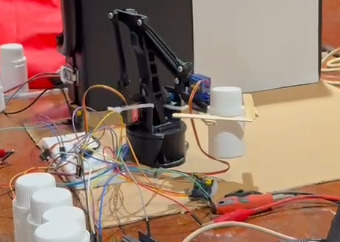
\includegraphics[width=0.88\textwidth]{gambar/robot_normal.jpeg}\\
    (a)
  \end{minipage}
  \vspace{1em}

  % Second image
  \begin{minipage}{\textwidth}
    \centering
    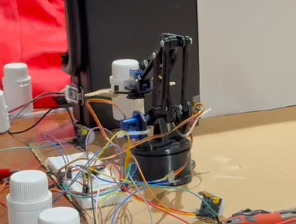
\includegraphics[width=0.88\textwidth]{gambar/robot_cacat.jpeg}\\
    (b)
  \end{minipage}
  \caption{Lengan robot menyortir kontainer: (a) normal, (b) cacat}
  \label{fig:robot-only}
  \vspace{-1em}
\end{figure}

Setelah lengan robot melepaskan kontainer di area penyortiran yang
telah ditentukan, sebuah sensor PIR yang terpasang di lokasi
tersebut akan mendeteksi keberadaan objek. Deteksi dari sensor PIR
ini berfungsi sebagai sinyal konfirmasi bahwa satu siklus penyortiran
telah selesai. Sinyal ini kemudian memicu pengiriman data hasil
klasifikasi, yang mencakup citra kontainer beserta label statusnya,
ke \textit{web server}. Untuk menampilkan informasi ini secara
\textit{real-time} kepada klien, sistem memanfaatkan protokol
\textit{WebSocket}. Tampilan \textit{website} dan hasil prediksi
dapat dilihat pada Gambar \ref{fig:web-test}.

\begin{figure}[H]
  \centering
  % First image
  \begin{minipage}{\textwidth}
    \centering
    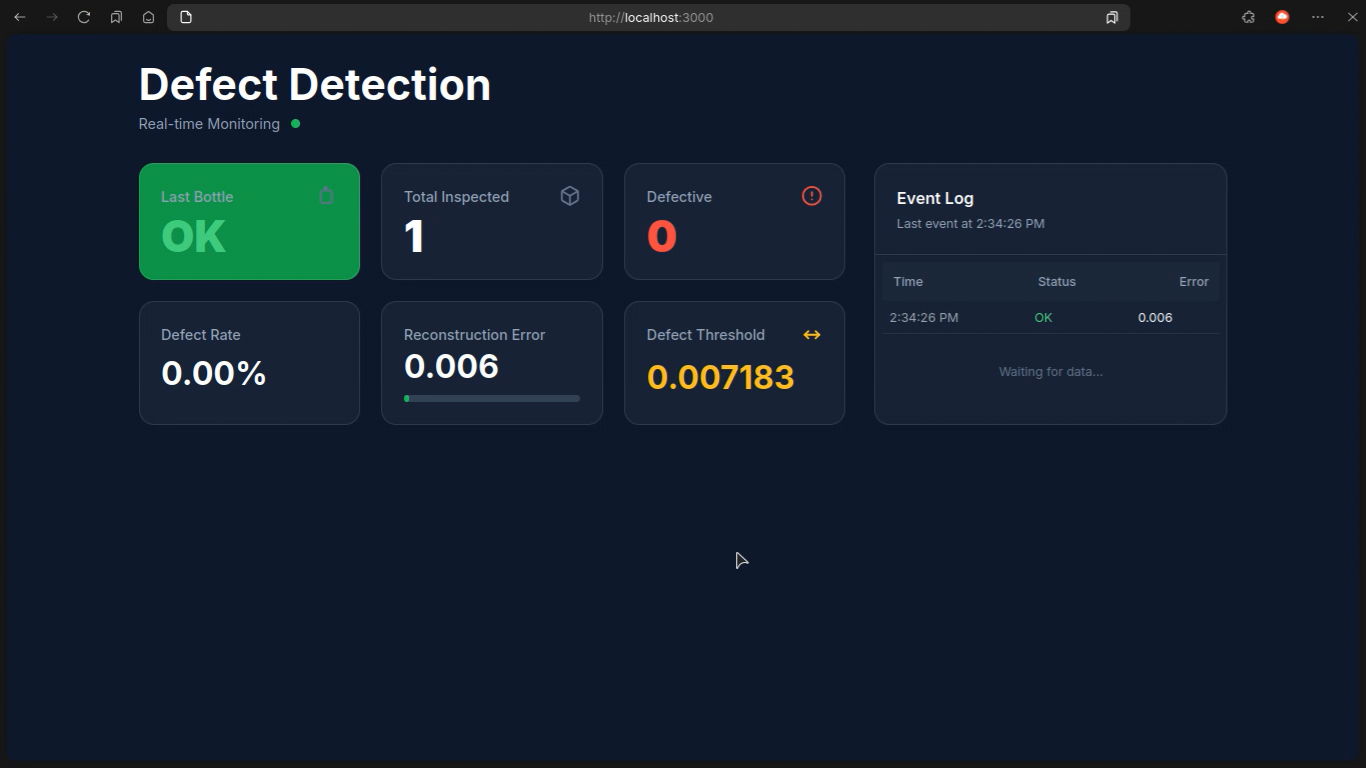
\includegraphics[width=\textwidth]{gambar/web_ss_normal.png}
    (a)
  \end{minipage}
  \vspace{1em}

  % Second image
  \begin{minipage}{\textwidth}
    \centering
    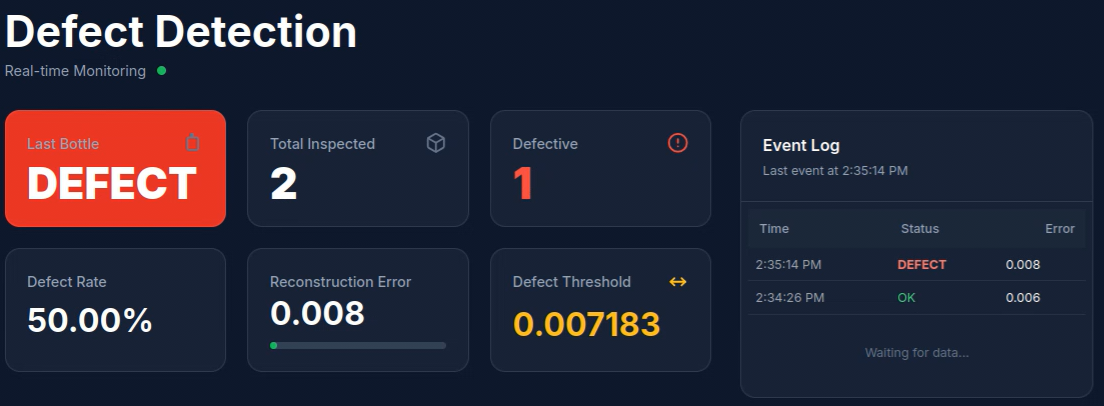
\includegraphics[width=\textwidth]{gambar/web_ss_cacat.png}
    (b)
  \end{minipage}
  \centering
  \caption{Tampilan hasil prediksi melalui \textit{website}: (a)
  kontainer normal, (b) kontainer cacat}
  \label{fig:web-test}
  \vspace{-1em}
\end{figure}

Untuk menguji keandalan dan konsistensi performa sistem, dilakukan
pengujian sebanyak 25 kali menggunakan sampel kontainer dengan
kondisi acak (normal dan cacat). Hasil kuantitatif dari setiap
pengujian ini dirangkum secara pada Tabel \ref{tab:error-samples-web}.

\begin{table}[H]
  \centering
  \caption{Nilai \textit{error} untuk setiap sampel uji}
  \label{tab:error-samples-web}
  \begin{tabular}{cccc}
    \toprule
    \textbf{No} & \textbf{Error} & \textbf{Kategori
      (Ambang Batas <
    0,007183)} & \textbf{Label Asli} \\
    \midrule
    1  & 0,006798 & Normal & Normal \\
    2  & 0,008298 & Cacat & Cacat \\
    3  & 0,006854 & Normal & Normal \\
    4  & 0,007066 & Normal & Normal \\
    5  & 0,006923 & Normal & Normal \\
    6  & 0,007607 & Cacat & Cacat \\
    7  & 0,007261 & Cacat & Cacat \\
    8  & 0,007393 & Cacat & Cacat \\
    9  & 0,006842 & Normal & Normal \\
    10 & 0,008099 & Cacat & Cacat \\
    11 & 0,006945 & Normal & Normal \\
    12 & 0,007381 & Cacat & Cacat \\
    13 & 0,006722 & Normal & Normal \\
    14 & 0,006865 & Normal & Normal \\
    15 & 0,007397 & Cacat & Cacat \\
    16 & 0,007099 & Normal & Normal \\
    17 & 0,006790 & Normal & Normal \\
    18 & 0,006760 & Normal & Normal \\
    19 & 0,007383 & Cacat & Cacat \\
    20 & 0,007693 & Cacat & Cacat \\
    21 & 0,008071 & Cacat & Cacat \\
    22 & 0,007977 & Cacat & Cacat \\
    23 & 0,006885 & Normal & Normal \\
    24 & 0,008007 & Cacat & Cacat \\
    25 & 0,006847 & Normal & Normal \\
    \midrule
    \multicolumn{3}{r}{\textbf{Tingkat Akurasi}} & \textbf{100\%} \\
    \bottomrule
  \end{tabular}
\end{table}

Hasil klasifikasi ditentukan berdasarkan perbandingan antara \textit{error}
rekonstruksi dengan ambang batas 0,007183. Sampel dengan \textit{error} lebih
rendah dikategorikan sebagai “Normal”, sedangkan yang lebih tinggi
dikategorikan sebagai “Cacat”. Dari Tabel 5 terlihat bahwa seluruh
prediksi model sesuai dengan kondisi sebenarnya (label asli),
menghasilkan tingkat akurasi 100\%. Contohnya, sampel no. 2 memiliki
nilai \textit{error} yang tinggi (0,008298) terklarifikasi dengan benar
”Cacat”. Sebaliknya sampel no. 1, dengan \textit{error} yang rendah
(0,006798) teklarifikasi dengan benar sebagai ”Normal”. Hasil
prediksi akhir pada \textit{website} ditunjukkan pada Gambar
\ref{fig:web-25}.

\begin{figure}[H]
  \centering
  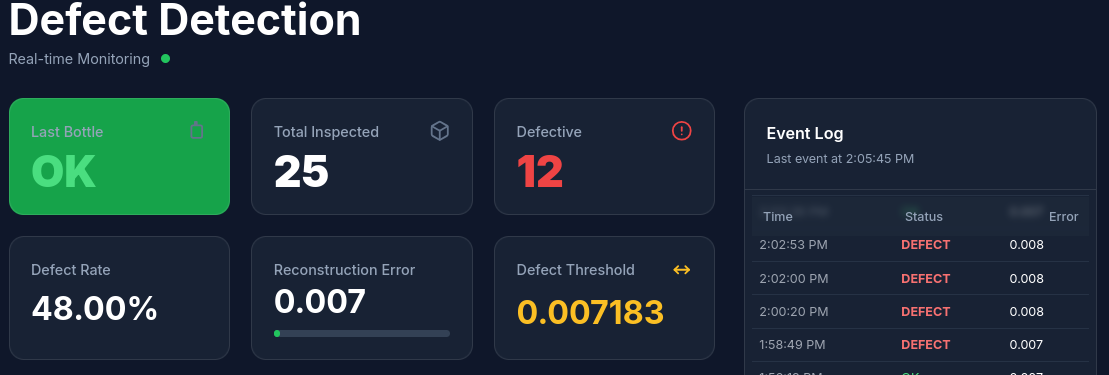
\includegraphics[width=\textwidth]{gambar/ss_web_25.png}
  \caption{Hasil prediksi kecacatan pada 25 sampel}
  \label{fig:web-25}
\end{figure}
\vspace{-1em}
